In this section, we introduce the problem of determining every location, here defined as the center and angle of rotation, of an ellipse with fixed shape parameters, such that it contains three given points.
This problem comes up in the development of an algorithm for MCER in the next section. 
It is important to point out that no prior studies were found on it, or even on related problems.
We propose an algorithm for it that involves determining the eigenvalues of a $6\times6$ complex matrix. We also analyze its efficiency in terms of numerical accuracy and display some solutions that it was able to obtain.

\subsection{Problem definition}

Given the shape parameters of an ellipse $(a, b) \in \R^2_{>0}$, $a > b$, and three points $u, v, w \in \R^2$, let $E\colon \R^2\times [0, \pi)\to{\color{blue}\mathcal{P}(\R^2)}$ be the coverage region of an ellipse with shape parameters $(a, b)$, we refer to the problem of obtaining $(q, \theta) \in \R^2\times [0, \pi)$, such that $\{u, v, w\} \subset \partial E(q, \theta)$ as Ellipse by Three Points Problem (E3P).
Because of its application here in our work, we are only interested in a method that can obtain every solution of E3P.

\subsection{Transforming E3P into a circle problem}

Initially, E3P is a problem of determining the values of three unknown continuous variables $(q_x, q_y)$, and $\theta$. However, as it will be shown, we can reduce this number to only one, as it is possible to obtain $q$ uniquely from $\theta$.
Let us assume that point $u$ is at the origin. If it is not, a simple translation by $-u$ applied to the three points can be made to put $u$ at the origin.
Assume as well that $(q, \theta)$ is a solution of E3P. 

Applying a rotation of $-\theta$ to the coordinate system makes the ellipse in the original solution become axis-parallel.
Then, that ellipse can be transformed into a circle of radius $b$ by squeezing the $x$-axis by $b/a$. This two-step transformation can be written as a function ${\color{blue}\varphi_\theta\colon \R^2 \to \R^2}$ defined as

\color{blue}
\begin{equation*}%\label{eq:trpnts}
\varphi_\theta(p)=\left[\begin{array}{cc}
\frac{b}{a}&0\\
0&1
\end{array}\right]
\left[\begin{array}{cc}
\cos{\theta}&\sin{\theta}\\
-\sin{\theta}&\cos{\theta}
\end{array}\right]\left[\begin{array}{c}
p_x\\
p_y
\end{array}\right].
\end{equation*}
\color{black}

An example of this transformation can be seen in \autoref{fig:circumscribed-circle}. As {\color{blue} $\varphi_\theta^{-1}$} is well-defined, instead of solving E3P, we can work with the univariate problem of determining an angle of rotation $\theta \in [0, \pi)$ that makes the triangle with vertices {\color{blue}$\varphi_\theta(u), \varphi_\theta(v), \varphi_\theta(w)$} be circumscribed in a circle of radius $b$. To make the notation less cluttered, we denote by $\Lambda(\theta)$ the triangle with vertices {\color{blue}$\varphi_\theta(u), \varphi_\theta(v), \varphi_\theta(w)$}.

\begin{figure}[!htb]
	\centering
	
	\includegraphics[scale=.8]{figures/circumscribed-circle}
	\caption{Transforming a solution of E3P into a solution of the circumcircle problem.}
	\label{fig:circumscribed-circle}
\end{figure}

As circles are uniquely defined by three non-collinear points, the circumcircle of $\Lambda(\theta)$ is unique, and its radius and center can be determined analytically \cite{weisstein}.
Let $|\Lambda(\theta)|$ denote the area of $\Lambda(\theta)$, using the formula from \cite[p.~189]{johnson1960} for the radius of a circumcircle of a triangle, and imposing that radius to be equal $b$, we define a function $\xi \colon [0, \pi) \to \R$ as
\begin{equation}\label{eq:xi}
\xi(\theta) = 16b^2|\Lambda(\theta)|^2 - \norm{{\color{blue}\varphi_\theta(v)}}^2\norm{{\color{blue}\varphi_\theta(w)}}^2\norm{{\color{blue}\varphi_\theta(v)}-{\color{blue}\varphi_\theta(w)}}^2,
\end{equation}
whose roots are angles of rotation which determine solutions of E3P through the inverse transformation {\color{blue}$\varphi_\theta^{-1}$}.
From a root $\hat{\theta}$ of $\xi$, let $\hat{q}$ be the center of the circumcircle of $\Lambda(\hat{\theta})$, the solution $({\color{blue}\varphi_{\hat{\theta}}^{-1}}(\hat{q}), \hat{\theta})$ of E3P is obtained. 

The algorithm for MCER described in the next section, of which E3P is a subproblem, goes through every solution of several instances of E3P. This is only possible if the number of solutions of E3P is finite, and it is only viable if that number is small. Next we introduce a lemma regarding that matter.

\begin{lem}\label{lema:e3p}
	E3P has at most six solutions.
\end{lem}

\begin{proof}
	The first thing to notice is that $\xi$ is a real trigonometric polynomial of degree $6$. 
	Its term of highest degree is the multiplication of the norms $\norm{{\color{blue}\varphi_\theta(v)}}^2\norm{{\color{blue}\varphi_\theta(w)}}^2\norm{{\color{blue}\varphi_\theta(v)}-{\color{blue}\varphi_\theta(w)}}^2$. In \cite[p.~150]{powell}, where a definition of real trigonometric polynomial is also given, it is stated that a $n$-degree real trigonometric polynomial can have up to $2n$ roots in $[0, 2\pi)$. Therefore, E3P has at most $12$ solutions in $[0, 2\pi]$.
	Half of these solutions, though, are duplicated as ellipses are symmetric to their axis.
\end{proof}

\subsection{Converting $\xi$ into a polynomial}

In \cite[p.~195]{horn}, a theorem is presented stating that for every univariate polynomial of degree $n$, there exists a companion matrix, which is a $n\times n$ matrix, such that its eigenvalues are the zeros of that polynomial. Finding every eigenvalue of a matrix can be done using the QR algorithm, which runs in $\bigO(n^3)$ and uses $\bigO(n^2)$ memory (a very complete introduction to it can be found in \cite{watkins:2008}). For example, for a {\color{blue} $4$-degree} polynomial $\sum_{k=0}^4 a_k x^4$, a possible companion matrix is given by

 \begin{equation*}
\left[\begin{array}{ccccc}
0 & 1 & 0 & 0\\
0 & 0 & 1 & 0\\
0 & 0 & 0 & 1\\
-\dfrac{a_0}{a_4} & -\dfrac{a_1}{a_4} & -\dfrac{a_2}{a_4} & -\dfrac{a_3}{a_4}
\end{array}\right].
\end{equation*}
In practice, we can use the very well-known LAPACK software library to obtain the eigenvalues of a matrix\cite{lapack}.
This approach works for both real or complex polynomials, and, because of that, based on \cite{weidner}, we describe a way of converting $\xi$ into a complex polynomial.

By using the identities $\cos{\theta} = (e^{i\theta} + e^{-i\theta})/2$, and $\sin{\theta} = (e^{i\theta} - e^{-i\theta})/(2i)$, which relate trigonometric functions with complex numbers in the unit circle $\mathbb{S}=\{z\in \mathbb{C}\colon |z|=1\}$, we can rewrite $\xi$ as a function of the variable $z=e^{i\theta}\in\mathbb{S}$. In \cite{weidner}, it is stated that this substitution when utilized for the task of determining the roots of a real trigonometric polynomial does not yield loss of accuracy.

As $\xi$ is a real trigonometric polynomial of degree $6$, $z$ appears with exponents from $-6$ up to $6$. Multiplying $\xi$ by $z^6$ and extending the domain of $z$ to $\mathbb{C}$, we obtain a complex polynomial $g(z)=\sum_{k=0}^{12} c_k z^k$, for some $c_0, \dots, c_{12} \in \mathbb{C}$. In practice, we utilize symbolic computation to obtain the actual coefficients of $g$ in terms of an instance of E3P.

Let $angle \colon \mathbb{C} \to [0, 2\pi)$ be a function that takes a complex number and returns its angle, then given a root $\hat{z}$ of $g$, if $|\hat{z}|=1$ and $angle(\hat{z}) \in [0, \pi)$, then $\hat{\theta} = angle(\hat{z})$ is a root of $\xi$. 

Observing that for any $z\in \mathbb{C}$, $angle(-z)=\pi+angle(z)$, and that for any ellipse the angles of rotation $\theta$ and $\theta + \pi$ are equivalent, we conclude that $g(-z)=g(z)$. This implies that all the odd-degree coefficients of $g$ are zero. Therefore, we can use the substitution $y=z^2$ to obtain a degree-$6$ polynomial $f(y)=\sum_{k=1}^6 c_{2k} y^k$ whose roots can be used to determine the roots of $\xi$: from a root $\hat{y}$ of $f$, $\hat{y}\in\mathbb{S}$, we have that $\hat{\theta}=angle(\hat{y})/2$ is a root of $\xi$.

Therefore, using the QR algorithm to obtain the eigenvalues of a companion matrix of the polynomial $f$, we can conclude that an algorithm to obtain every solution of E3P can be implemented, and that such algorithm takes a constant number of operations to do so.

%Lastly, It worth mentioning that a pattern on the coefficients of $f$ was identified, and maybe it can be used for further improvements. Analyzing the polynomials produced for several instances, we observed that $c_k = \overline{c_{6-k}}$, for all $k=0\dots 6$.

\subsection{Choosing a precision constant}

In this section, we describe an experiment we made to choose a precision constant for comparing if a root of $f$ returned as an eigenvalue of its companion matrix is in the unit circle. The implementation was coded in C++, and LAPACK's ZGEEV was utilized to obtain the eigenvalues of the companion matrix of $f$ (more information about the implementation is given in Section~\ref{section:implementation}). For the experiment, we defined $K\in\R$, $K>0$, and considered instances with the ellipse's shape parameters $(K, \frac{K}{2})$, for $K\in\{10^j\colon j=0,\dots,10\}$.

The experiment considered instances of E3P where the three points are vertices of an ellipse rotated by $\theta\in[0, \pi)$. Such instances only have one solution, and therefore, roots with multiplicity greater than one are expected.
For each value of $K$, we ran the algorithm for $100$ instances generated randomly by sampling $\theta$ according to a uniform distribution. For each instance, we took the root $\hat{z}$ which produced the closest solution to the known one. Then, for each $K$, as it can be seen in \autoref{fig:e3p_known_sols2}, we considered the maximum and the average distance to the unit circle $|1-|\hat{z}||$; and, as it presented in \autoref{fig:e3p_known_sols1}, the maximum and average error $|f(\hat{z})|$.

From this experiment, we decided to adopt a precision constant of $10^{-6}$ to consider a root of $f$ to be in the unit circle, and as an additional check, we adopted a precision constant of $10^{-9}$ to consider a root to be a solution of E3P.

\begin{figure}[!htb]
	
	\begin{subfigure}{.5\textwidth}
		\centering

		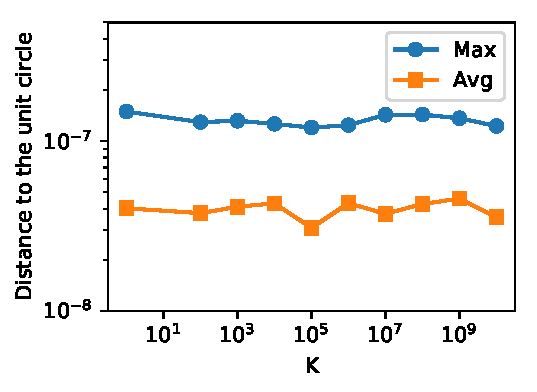
\includegraphics[scale=.8]{figures/e3p_known_sols2}
		\caption{}
		\label{fig:e3p_known_sols2}
	\end{subfigure}
	\begin{subfigure}{.5\textwidth}
	\centering
	
	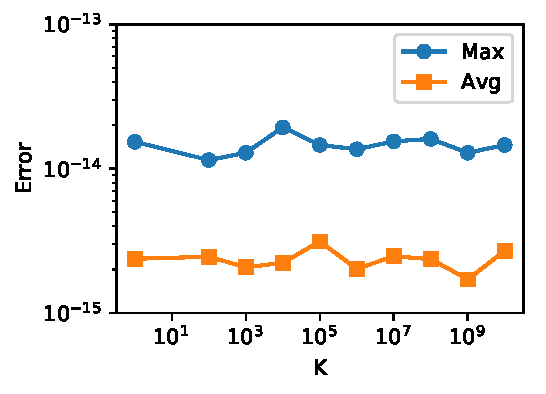
\includegraphics[scale=.8]{figures/e3p_known_sols1}
	\caption{}
	\label{fig:e3p_known_sols1}
	\end{subfigure}
\caption{(a) Shows the maximum and average distance to the unit circle $|1-|\hat{z}||$. (b) Shows the maximum and average error $|f(\hat{z})|$.}
\end{figure}

\subsection{Instances with four and six solutions}

Any instance of E3P, as stated by \autoref{lema:e3p}, can have up to six solutions. At first, though, this bound seemed to be loose as for randomly generated instances, we were not able to obtain instances with more than two solutions.

After some investigation, we were able to construct some four-solution instances (an example is displayed in \autoref{fig:e3p_4sols}). An interesting property of those solutions is that their three points form an isosceles triangle.

\begin{figure}[!htb]
	\begin{subfigure}{.5\textwidth}
		\centering
		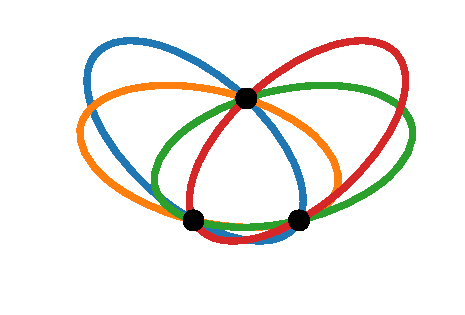
\includegraphics[scale=.9]{figures/e3p_4sols}
		\caption{}
		\label{fig:e3p_4sols}
	\end{subfigure}
	\begin{subfigure}{.5\textwidth}
		\centering
		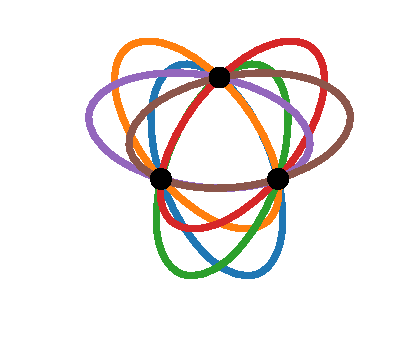
\includegraphics[scale=.9]{figures/e3p_6sols}
		\caption{}
		\label{fig:e3p_6sols}
	\end{subfigure}
\caption{(a) The four solutions for an instance of E3P where the three points form an isosceles triangle. (b) The six solutions for an instance of E3P where the three points form an equilateral triangle.}
\end{figure}

Six-solution instances were found by taking a particular case of the four-solution instances, we took the three points as the vertices of a equilateral triangle. An example of that is shown in \autoref{fig:e3p_6sols}.

It should be pointed out that neither non-isosceles instances with four solutions nor non-equilateral instances with six solutions could be found. Further investigating these possible properties of E3P is left as future work.
